\chapter{Le singulet, l’inégalité de Bell et l’impossibilité de la clonation}

\lectureoverview{Un signe moins relatif transforme un état de deux spins simplement corrélés en singulet invariant par rotation. Nous identifions cet état en calculant le spin total, nous nous servons de son anticorrélation parfaite pour formuler une expérience de Bell, puis nous traduisons des propositions classiques en opérateurs de projection quantiques. Les probabilités qui en résultent violent l’inégalité de dénombrement classique de Bell. Les questions de localité, de synchronisation des mesures et d’incertitude conduisent ensuite à une seconde conséquence de la mécanique quantique linéaire : un état inconnu ne peut pas être copié par une machine universelle de clonation.}

\section{Quelle différence un signe peut-il faire ?}

Considérons deux électrons et omettons le symbole du produit tensoriel dans les états de base :
\begin{equation}
  \ket{ud}\equiv\ket{u}_1\otimes\ket{d}_2,
  \qquad
  \ket{du}\equiv\ket{d}_1\otimes\ket{u}_2.
\end{equation}
Deux superpositions particulièrement simples ne diffèrent que par un signe,
\begin{equation}
  \ket{\psi_\pm}
  =
  \frac{\ket{ud}\pm\ket{du}}{\sqrt2}.
  \label{eq:l05-two-signs}
\end{equation}
Le facteur \(1/\sqrt2\) assure que la probabilité totale vaut un. Dans les deux états, une mesure suivant le troisième axe donne des résultats opposés : si l’électron 1 est dans l’état haut, l’électron 2 est dans l’état bas, et inversement. Cette seule corrélation ne permet donc pas de détecter le signe. Les deux états sont néanmoins physiquement différents.

Nous utiliserons à plusieurs reprises les actions des matrices de Pauli :
\begin{align}
  \sigma_1\ket{u}&=\ket{d},&
  \sigma_1\ket{d}&=\ket{u},\nonumber\\
  \sigma_2\ket{u}&=i\ket{d},&
  \sigma_2\ket{d}&=-i\ket{u},\nonumber\\
  \sigma_3\ket{u}&=\ket{u},&
  \sigma_3\ket{d}&=-\ket{d}.
  \label{eq:l05-pauli-actions}
\end{align}
Nous réservons \(\sigma_i\) aux opérateurs agissant sur l’électron 1 et introduisons une famille identique, \(\tau_i\), agissant sur l’électron 2.

\begin{figure}[htbp]
\centering
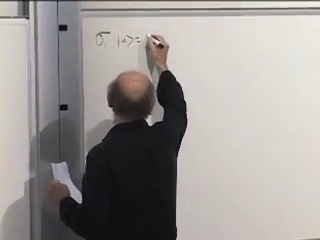
\includegraphics[width=0.62\linewidth]{lecture_05_figure_02.png}
\caption{Tableau complet des actions des matrices de Pauli utilisé dans toute la comparaison.}
\lectureframe{00:03:15}
\end{figure}

Dans aucun des deux états, le spin de l’une ou l’autre particule n’a de direction privilégiée :
\begin{equation}
  \expect{\sigma_i}_{\psi_\pm}=0,
  \qquad
  \expect{\tau_i}_{\psi_\pm}=0,
  \qquad i=1,2,3.
  \label{eq:l05-local-zero}
\end{equation}
Par exemple, le calcul explicite demandé pour l’état plus donne
\begin{align}
  \bra{\psi_+}\sigma_3\ket{\psi_+}
  &=
  \frac12
  \bigl(\bra{ud}+\bra{du}\bigr)
  \bigl(\ket{ud}-\ket{du}\bigr)\nonumber\\
  &=
  \frac12(1-1)=0.
  \label{eq:l05-sigma3-expectation}
\end{align}
Les termes croisés s’annulent parce que \(\braket{ud}{du}=0\).

\begin{figure}[htbp]
\centering
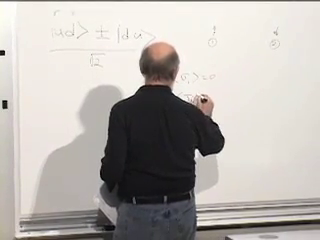
\includegraphics[width=0.78\linewidth]{lecture_05_figure_03.png}
\caption{Calcul de la valeur moyenne dans l’état plus en faisant agir \(\sigma_3\) et en utilisant l’orthogonalité.}
\lectureframe{00:07:00}
\end{figure}

\begin{classroomqa}
\lecturetimestamp{00:07:13}
\audiencequestion{Une valeur moyenne nulle signifie-t-elle qu’on peut mesurer une valeur nulle pour un spin individuel ?}
\lecturerresponse{Non. La mesure d’une composante du spin ne peut donner que \(+1\) ou \(-1\) ; \(\sigma_i\) n’a pas de valeur propre nulle. L’équation~\eqref{eq:l05-local-zero} signifie que des mesures répétées donnent les résultats d’un tirage à pile ou face, et non que chaque résultat individuel est nul.}
\end{classroomqa}

Le premier critère de distinction plausible ne nous a donc pas permis de trancher. Les valeurs moyennes locales ne révèlent pas le signe relatif ; il faut mesurer une propriété de la paire.

\section{Le spin total sélectionne le singulet}

Le moment magnétique de la paire est représenté par la somme vectorielle
\begin{equation}
  \boldsymbol{\Sigma}
  =
  \boldsymbol{\sigma}+\boldsymbol{\tau}.
\end{equation}
Sa troisième composante annule les deux vecteurs de base :
\begin{align}
  (\sigma_3+\tau_3)\ket{ud}
  &=(1-1)\ket{ud}=0,\nonumber\\
  (\sigma_3+\tau_3)\ket{du}
  &=(-1+1)\ket{du}=0.
\end{align}
Par conséquent,
\begin{equation}
  (\sigma_3+\tau_3)\ket{\psi_\pm}=0.
\end{equation}
Pour les deux choix de signe, la composante totale suivant le troisième axe est nulle à chaque mesure.

La première composante permet de les distinguer. D’après l’équation~\eqref{eq:l05-pauli-actions},
\begin{align}
  (\sigma_1+\tau_1)\ket{ud}
  &=\ket{dd}+\ket{uu},\nonumber\\
  (\sigma_1+\tau_1)\ket{du}
  &=\ket{uu}+\ket{dd}.
\end{align}
On obtient donc
\begin{align}
  (\sigma_1+\tau_1)\ket{\psi_+}
  &=
  \sqrt2\bigl(\ket{uu}+\ket{dd}\bigr),\nonumber\\
  (\sigma_1+\tau_1)\ket{\psi_-}
  &=0.
  \label{eq:l05-total-x}
\end{align}
La valeur moyenne de cette observable peut être nulle dans l’état plus, mais celui-ci n’est pas son état propre de valeur propre nulle.

\begin{classroomqa}
\lecturetimestamp{00:13:02}
\audiencequestion{Quels résultats la composante totale peut-elle donner si elle n’annule pas l’état ?}
\lecturerresponse{Chaque spin individuel donne \(+1\) ou \(-1\) ; leur somme peut donc valoir \(2\), \(0\) ou \(-2\). Une valeur moyenne nulle n’impose pas un résultat nul à chaque mesure.}
\end{classroomqa}

La deuxième composante complète le test. Les facteurs de \(i\) se compensent dans la combinaison antisymétrique :
\begin{equation}
  (\sigma_2+\tau_2)\ket{\psi_-}=0.
\end{equation}
Les trois composantes annulent donc l’état moins,
\begin{equation}
  \bigl(\boldsymbol{\sigma}+\boldsymbol{\tau}\bigr)
  \cdot\hat n\,\ket{\psi_-}=0
  \qquad\text{for every unit vector }\hat n.
  \label{eq:l05-singlet-any-axis}
\end{equation}

\begin{figure}[htbp]
\centering
\includegraphics[width=0.84\linewidth]{lecture_05_figure_06.png}
\caption{Les annulations, composante par composante, qui identifient l’état moins comme un état de spin total nul.}
\lectureframe{00:16:30}
\end{figure}

L’état antisymétrique \(\ket{\psi_-}\) est le \emph{singulet}. Il est invariant par rotation : quel que soit l’axe, le spin total mesuré vaut zéro. L’état symétrique de l’équation~\eqref{eq:l05-two-signs} appartient au secteur triplet.

\begin{classroomqa}
\lecturetimestamp{00:19:06}
\audiencequestion{Le résultat de spins opposés n’est-il vrai qu’en moyenne ?}
\lecturerresponse{Pour le singulet, il est vrai à chaque mesure. L’équation~\eqref{eq:l05-singlet-any-axis} est une équation aux vecteurs propres ; mesurer la même composante sur les deux particules donne donc toujours des résultats dont la somme est la valeur propre zéro.}
\end{classroomqa}

\begin{classroomqa}
\lecturetimestamp{00:19:36}
\audiencequestion{Pourquoi appelle-t-on l’autre état un triplet ?}
\lecturerresponse{Ce nom vient des trois états du multiplet de spin total un. Sa dérivation est reportée à plus tard ; le calcul présent requiert seulement de distinguer l’état symétrique du secteur singulet, qui est de dimension un.}
\end{classroomqa}

Si Bob mesure une composante quelconque de son électron, il sait immédiatement quel résultat Alice obtiendrait en mesurant la même composante sur le sien : elle doit obtenir le résultat opposé. C’est une corrélation d’Einstein--Podolsky--Rosen. Deux pièces cachées peuvent elles aussi porter des résultats opposés, mais pour une seule question convenue à l’avance. Le singulet, lui, fournit une anticorrélation parfaite, quel que soit l’axe spatial choisi.

\begin{classroomqa}
\lecturetimestamp{00:20:55}
\audiencequestion{Einstein, Podolsky et Rosen ont-ils découvert l’intrication ?}
\lecturerresponse{Non. Schrödinger a étudié le phénomène et introduit le vocabulaire de l’intrication. L’argument EPR a mis en évidence avec une acuité particulière le problème des corrélations à distance.}
\end{classroomqa}

\begin{classroomqa}
\lecturetimestamp{00:23:50}
\audiencequestion{Cette corrélation immédiate viole-t-elle la causalité ? Et l’ordre des mesures dépend-il de l’observateur ?}
\lecturerresponse{Aucun message exploitable n’est transmis. Les résultats locaux d’Alice restent équiprobables, que Bob effectue une mesure ou non, quel que soit l’ordre des événements dans les référentiels inertiels. Elle ne peut vérifier la corrélation qu’après avoir reçu le résultat de Bob par un canal classique ordinaire, qui ne peut pas dépasser la vitesse de la lumière.}
\end{classroomqa}

\section{L’inégalité de Bell relève du dénombrement classique}

La portée du résultat de Bell peut sembler changer selon les jours. Parfois, il paraît révéler le trait le plus profond de la mécanique quantique ; d’autres fois, il semble n’être qu’une conséquence inévitable de son formalisme. Bell lui-même, comme Feynman, pouvait défendre ces deux points de vue. L’inégalité, cependant, est élémentaire. C’est sa violation qui surprend.

Considérons un ensemble ordinaire d’objets. Chacun peut posséder ou non trois propriétés, \(A\), \(B\) et \(C\). Notons \(N(A,\neg B)\) le nombre de ceux qui possèdent \(A\) mais pas \(B\). La logique classique des ensembles implique
\begin{equation}
  N(A,\neg B)+N(B,\neg C)
  \geq
  N(A,\neg C).
  \label{eq:l05-bell-count}
\end{equation}
La démonstration repose sur l’inclusion d’ensembles
\begin{equation}
  A\cap C^{c}
  \subseteq
  (A\cap B^{c})\cup(B\cap C^{c}).
  \label{eq:l05-set-inclusion}
\end{equation}
En effet, un élément de \(A\cap C^c\) appartient ou non à \(B\). Dans le premier cas, il appartient à \(B\cap C^c\) ; dans le second, il appartient à \(A\cap B^c\). Dénombrer la réunion ne peut qu’ajouter des éléments à l’ensemble de gauche.

\begin{figure}[htbp]
\centering
\includegraphics[width=0.78\linewidth]{lecture_05_figure_07.png}
\caption{La démonstration au tableau décompose trois sous-ensembles classiques qui se recouvrent en régions de cardinal non négatif.}
\lectureframe{00:31:15}
\end{figure}

On peut aussi désigner les régions disjointes du diagramme des trois ensembles par des entiers non négatifs \(N_i\). Les deux membres de l’équation~\eqref{eq:l05-bell-count} contiennent les régions qui constituent \(A\cap C^c\), mais le membre de gauche en contient d’autres, de cardinal non négatif. Rien de quantique n’intervient ici. C’est un théorème sur les sous-ensembles et les alternatives logiques ordinaires.

\section{Du raisonnement ensembliste à l’expérience de spin}

Préparons de nombreuses paires d’électrons indépendantes dans l’état singulet et définissons trois propositions concernant l’électron 1 :
\begin{align}
  A&:\ \text{spin 1 is up at }0^\circ\text{, along the third axis},\nonumber\\
  B&:\ \text{spin 1 is up at }45^\circ\text{ in the }zx\text{-plane},\nonumber\\
  C&:\ \text{spin 1 is up at }90^\circ\text{, along the first axis}.
  \label{eq:l05-abc}
\end{align}

\begin{figure}[htbp]
\centering
\includegraphics[width=0.82\linewidth]{lecture_05_figure_08.png}
\caption{Les trois propositions sur le spin sont fixées aux angles \(0^\circ\), \(45^\circ\) et \(90^\circ\) dans un même plan.}
\lectureframe{00:39:00}
\end{figure}

Dans l’état singulet, la négation d’une proposition sur l’électron 1 peut se réécrire comme une proposition positive sur l’électron 2. Par exemple,
\begin{align}
  \neg B
  &:\ \text{spin 1 is down at }45^\circ\nonumber\\
  &\Longleftrightarrow
  \text{spin 2 is up at }45^\circ.
\end{align}
De même, \(\neg C\) devient l’énoncé selon lequel l’électron 2 est dans l’état haut à \(90^\circ\).

\begin{classroomqa}
\lecturetimestamp{00:40:04}
\audiencequestion{Est-ce que \(\neg C\) signifie que l’électron 2 est dans l’état bas à \(90^\circ\) ?}
\lecturerresponse{Non. Il faut d’abord nier \(C\) : l’électron 1 est dans l’état bas à \(90^\circ\). L’anticorrélation parfaite du singulet implique alors que l’électron 2 est dans l’état haut le long de ce même axe. Il faut distinguer ces deux inversions.}
\end{classroomqa}

Pour un grand ensemble, les nombres et les probabilités ne diffèrent que par le facteur commun correspondant au nombre de paires préparées. L’invariance par rotation donne aussi
\begin{equation}
  P(A,\neg B)=P(B,\neg C),
\end{equation}
car la deuxième expérience s’obtient en faisant subir une rotation de \(45^\circ\) à la première. L’inégalité classique de Bell imposerait donc
\begin{equation}
  2P(A,\neg B)\geq P(A,\neg C).
  \label{eq:l05-bell-probability}
\end{equation}
Il nous faut maintenant une méthode efficace pour calculer ces probabilités.

\section{Les propositions deviennent des projecteurs}

Dans un espace vectoriel ordinaire à trois dimensions, un projecteur supprime toute composante perpendiculaire au sous-espace choisi. Un projecteur de dimension un projette orthogonalement un vecteur sur une droite ; un projecteur de dimension deux le projette sur un plan. Si \(P\) projette sur un sous-espace donné,
\begin{equation}
  P\ket{\alpha}=\ket{\alpha_P}.
\end{equation}

\begin{figure}[htbp]
\centering
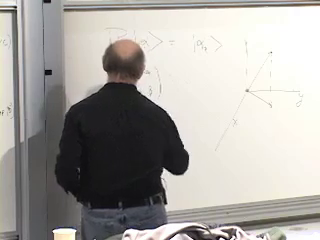
\includegraphics[width=0.76\linewidth]{lecture_05_figure_04.png}
\caption{La projection géométrique et sa notation opératorielle sont présentées côte à côte.}
\lectureframe{00:49:53}
\end{figure}

\begin{figure}[htbp]
\centering
\begin{tikzpicture}[scale=1.05,>=Latex]
  \draw[->] (-0.25,0)--(4.0,0);
  \draw[thick] (-0.25,-0.25)--(3.55,2.6);
  \draw[->,very thick] (0,0)--(2.25,3.05)
    node[above] {\(\ket{\alpha}\)};
  \coordinate (P) at (2.72,1.98);
  \draw[dashed] (2.25,3.05)--(P);
  \draw[->,very thick] (0,0)--(P)
    node[right] {\(\ket{\alpha_P}\)};
  \node[below right] at (3.1,2.25) {projected subspace};
\end{tikzpicture}
\caption{Reconstruction nette de la géométrie de la projection.}
\end{figure}

Dans l’espace de Hilbert d’un spin, la proposition \(\sigma_3=+1\) correspond au sous-espace de dimension un engendré par \(\ket{u}\). Le projecteur correspondant agit ainsi :
\begin{equation}
  P_{\sigma_3=+1}
  \begin{pmatrix}\alpha\\\beta\end{pmatrix}
  =
  \begin{pmatrix}\alpha\\0\end{pmatrix},
  \qquad
  P_{\sigma_3=-1}
  \begin{pmatrix}\alpha\\\beta\end{pmatrix}
  =
  \begin{pmatrix}0\\\beta\end{pmatrix}.
  \label{eq:l05-projector-actions}
\end{equation}

\begin{classroomqa}
\lecturetimestamp{00:49:55}
\audiencequestion{Le premier projecteur indique-t-il jusqu’où le vecteur s’élève sur un axe vertical ?}
\lecturerresponse{Non. Il élimine simplement le coefficient orthogonal \(\beta\). Les composantes sont des amplitudes dans l’espace de Hilbert, et non des coordonnées spatiales ordinaires du spin.}
\end{classroomqa}

\begin{figure}[htbp]
\centering
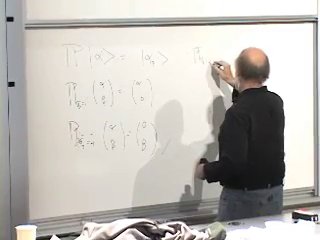
\includegraphics[width=0.78\linewidth]{lecture_05_figure_05.png}
\caption{Les projecteurs agissent d’abord sur un spineur général, puis sont écrits sous forme de matrices explicites.}
\lectureframe{00:51:40}
\end{figure}

La forme matricielle est
\begin{equation}
  P_{\sigma_3=+1}
  =
  \begin{pmatrix}1&0\\0&0\end{pmatrix}
  =
  \frac{I+\sigma_3}{2}.
  \label{eq:l05-p3}
\end{equation}
La même construction s’applique suivant n’importe quel vecteur unitaire \(\hat n\) :
\begin{equation}
  P_{\boldsymbol{\sigma}\cdot\hat n=+1}
  =
  \frac{I+\boldsymbol{\sigma}\cdot\hat n}{2}.
  \label{eq:l05-pn}
\end{equation}

\begin{classroomqa}
\lecturetimestamp{00:53:09}
\audiencequestion{Quel est le projecteur sur \(\sigma_1=+1\) ?}
\lecturerresponse{Dans l’équation~\eqref{eq:l05-p3}, remplaçons \(\sigma_3\) par \(\sigma_1\) : \(P_{\sigma_1=+1}=(I+\sigma_1)/2\).}
\end{classroomqa}

La règle de Born s’écrit alors utilement en termes de propositions :
\begin{equation}
  P(\mathcal A\text{ is true in }\ket{\psi})
  =
  \bra{\psi}P_{\mathcal A}\ket{\psi}.
  \label{eq:l05-projector-born}
\end{equation}
Pour un spineur normalisé \(\ket{\psi}=(\alpha,\beta)^T\), l’équation~\eqref{eq:l05-projector-born} donne, avec \(P_{\sigma_3=+1}\), \(|\alpha|^2\), comme il se doit.

Cette formulation met en évidence la différence entre les propositions classiques et quantiques. En logique classique, une propriété correspond à un sous-ensemble d’un ensemble. En mécanique quantique, une propriété correspond à un sous-espace de l’espace de Hilbert, ou, de façon équivalente, à son projecteur. Les sous-ensembles et les sous-espaces vectoriels n’obéissent pas aux mêmes opérations de treillis ; c’est de cette différence que naît la contradiction de Bell.

\subsection{Le projecteur conjoint de Bell}

Pour \(A\wedge\neg B\), l’électron 1 doit être dans l’état haut suivant le troisième axe, et l’électron 2 doit être dans l’état haut suivant
\begin{equation}
  \hat n_{45}=\frac{\hat x+\hat z}{\sqrt2}.
\end{equation}
La composante pertinente du spin de la deuxième particule est
\begin{equation}
  \boldsymbol{\tau}\cdot\hat n_{45}
  =
  \frac{\tau_1+\tau_3}{\sqrt2}.
\end{equation}
Le projecteur conjoint est donc
\begin{equation}
  P_{A\wedge\neg B}
  =
  \frac{I+\sigma_3}{2}
  \frac{I+(\tau_1+\tau_3)/\sqrt2}{2}.
  \label{eq:l05-joint-projector}
\end{equation}

\begin{classroomqa}
\lecturetimestamp{00:59:18}
\audiencequestion{Pourquoi la composante de spin à \(45^\circ\) comporte-t-elle un facteur \(1/\sqrt2\) ?}
\lecturerresponse{La direction doit être un vecteur unitaire. Ses composantes suivant le premier et le troisième axe valent toutes deux \(1/\sqrt2\) ; l’observable correspondante est donc \((\tau_1+\tau_3)/\sqrt2\).}
\end{classroomqa}

\begin{classroomqa}
\lecturetimestamp{01:00:52}
\audiencequestion{L’expression entière \(I+\boldsymbol{\tau}\cdot\hat n_{45}\) est-elle divisée par deux ?}
\lecturerresponse{Oui. Le projecteur est \(\bigl(I+\boldsymbol{\tau}\cdot\hat n_{45}\bigr)/2\) ; le facteur \(1/2\) multiplie le numérateur entier.}
\end{classroomqa}

Les deux facteurs de l’équation~\eqref{eq:l05-joint-projector} agissent sur des facteurs tensoriels différents et commutent. Leur produit annule d’abord toute composante où l’électron 1 est dans l’état bas, puis toute composante restante où l’électron 2 est dans l’état bas suivant \(\hat n_{45}\).

\section{Les nombres quantiques inversent l’inégalité}

Notons
\begin{equation}
  \ket{\psi_s}
  =
  \frac{\ket{ud}-\ket{du}}{\sqrt2}
\end{equation}
le singulet. Commençons par
\begin{equation}
  P(A,\neg B)
  =
  \bra{\psi_s}P_{A\wedge\neg B}\ket{\psi_s}.
\end{equation}
Le facteur \((I+\sigma_3)/2\) annule \(\ket{du}\) et laisse \(\ket{ud}/\sqrt2\). Le deuxième facteur donne alors
\begin{align}
  \frac{I+(\tau_1+\tau_3)/\sqrt2}{2}\ket{ud}
  &\notag\\[-0.3em]
  &=
  \frac12
  \left[
    \ket{ud}
    +\frac{\ket{uu}-\ket{ud}}{\sqrt2}
  \right]\nonumber\\
  &=
  \frac12
  \Biggl[
    \left(1-\frac1{\sqrt2}\right)\ket{ud}
  \nonumber\\
  &\qquad
    +\frac1{\sqrt2}\ket{uu}\Biggr].
  \label{eq:l05-projector-action}
\end{align}
Le terme \(\ket{uu}\) a un recouvrement nul avec le bra singulet ; les facteurs de normalisation restants donnent
\begin{equation}
  P(A,\neg B)
  =
  \frac14\left(1-\frac1{\sqrt2}\right).
  \label{eq:l05-pab}
\end{equation}

\begin{figure}[htbp]
\centering
\includegraphics[width=0.88\linewidth]{lecture_05_figure_09.png}
\caption{Le calcul avec le projecteur conserve le recouvrement de \(\ket{ud}\) et élimine la contribution orthogonale de \(\ket{uu}\).}
\lectureframe{01:08:20}
\end{figure}

L’invariance par rotation donne le même résultat pour la paire de directions suivante :
\begin{equation}
  P(B,\neg C)
  =
  \frac14\left(1-\frac1{\sqrt2}\right).
\end{equation}
Pour \(A\wedge\neg C\), le deuxième axe coïncide avec le premier axe spatial, donc
\begin{equation}
  P_{A\wedge\neg C}
  =
  \frac{I+\sigma_3}{2}\frac{I+\tau_1}{2}.
\end{equation}
Le premier facteur laisse à nouveau \(\ket{ud}/\sqrt2\). Le terme \(\tau_1\) produit \(\ket{uu}\), qui est orthogonal au bra singulet, tandis que le terme identité subsiste. Ainsi,
\begin{equation}
  P(A,\neg C)=\frac14.
  \label{eq:l05-pac}
\end{equation}
En réunissant les trois résultats,
\begin{equation}
  \underbrace{
  P(A,\neg B)+P(B,\neg C)
  }_{\frac12(1-1/\sqrt2)\approx0.146}
  <
  \underbrace{
  P(A,\neg C)
  }_{\frac14=0.25}.
  \label{eq:l05-bell-violation}
\end{equation}

\begin{figure}[htbp]
\centering
\includegraphics[width=0.84\linewidth]{lecture_05_figure_10.png}
\caption{Le calcul complet au tableau fait apparaître le membre de gauche, plus petit, et le membre de droite, plus grand, de l’inégalité de Bell.}
\lectureframe{01:12:15}
\end{figure}

L’équation~\eqref{eq:l05-bell-violation} inverse l’équation~\eqref{eq:l05-bell-probability}. Il ne s’ensuit pas que la mécanique quantique se contredise. Cela signifie que les corrélations du singulet ne peuvent provenir d’un modèle classique local où les trois propositions sur le spin auraient des valeurs de vérité ordinaires, au sens de la théorie des ensembles, indépendantes du choix de mesure effectué à distance. Une simulation classique ne peut reproduire ces corrélations qu’en abandonnant au moins une hypothèse de Bell, en particulier la localité.

\section{Ce que teste l’expérience de Bell}

La mécanique quantique prédit déjà la violation. Une expérience doit aussi écarter la possibilité classique qu’un détecteur informe l’autre du réglage choisi ou du résultat obtenu. Les deux appareils doivent être assez éloignés, et les choix et détections assez rapprochés dans le temps, pour qu’un signal lumineux ne puisse passer de l’un à l’autre. L’expérience d’Aspect a rendu convaincantes, dans les faits, la synchronisation et l’isolation des appareils.

\begin{classroomqa}
\lecturetimestamp{01:13:15}
\audiencequestion{Si la mécanique quantique donne déjà la réponse, les expériences de Bell nous ont-elles appris quelque chose ?}
\lecturerresponse{Elles ont vérifié que la nature suit la prédiction quantique dans cette expérience précise de corrélation et, point crucial, rendu les deux appareils de mesure indépendants pendant le temps nécessaire à la propagation de la lumière. La maîtrise expérimentale et la synchronisation constituaient en elles-mêmes des avancées considérables.}
\end{classroomqa}

\begin{classroomqa}
\lecturetimestamp{01:18:19}
\audiencequestion{Qu’a apporté Bell après la discussion d’Einstein sur l’action fantomatique à distance ?}
\lecturerresponse{Bell a établi une inégalité quantitative. Il a défini une expérience de corrélation réalisable dont la prédiction quantique exclut une explication sous-jacente classique et locale, au lieu de s’en tenir à un malaise d’ordre philosophique. Bell est resté partagé sur le caractère inévitable ou profond de ce résultat et s’est montré de plus en plus disposé à remettre en question la mécanique quantique standard.}
\end{classroomqa}

Les particules peuvent être séparées par des kilomètres tout en partageant un même état conjoint, mais il s’agit toujours d’une expérience quantique sur de petits systèmes. Les interactions avec l’environnement tendent à détruire les relations de phase nécessaires. Les molécules d’air, les photons parasites et les perturbations thermiques peuvent s’intriquer avec la paire ; il faut donc effectuer la séparation dans un environnement froid et bien isolé.

\begin{classroomqa}
\lecturetimestamp{01:19:53}
\audiencequestion{Un état commun étendu sur une grande distance fait-il de cette paire un objet quantique macroscopique ?}
\lecturerresponse{Il vaut mieux parler de petits systèmes quantiques éloignés l’un de l’autre. Leur séparation peut être grande, mais la préservation de leur fonction d’onde conjointe devient de plus en plus délicate, car les interactions incontrôlées avec l’environnement détruisent la cohérence utile. Deux boules de bowling ordinaires ne permettent pas la même expérience.}
\end{classroomqa}

\begin{classroomqa}
\lecturetimestamp{01:21:23}
\audiencequestion{La mesure d’une particule peut-elle révéler une information complémentaire sur l’autre et permettre ainsi de contourner le principe d’incertitude ?}
\lecturerresponse{On peut mesurer, par exemple, la position d’une particule et la quantité de mouvement de l’autre. Ce n’est pas une mesure simultanée d’observables qui ne commutent pas sur une même particule. La restriction due à l’incertitude pour un système unique n’a pas été contournée.}
\end{classroomqa}

\section{Quand un produit signifie-t-il « et » ?}

Dans le calcul de Bell, nous avons multiplié deux projecteurs. Cette opération représente une conjonction seulement pour des propositions compatibles.

\begin{classroomqa}
\lecturetimestamp{01:22:39}
\audiencequestion{Pourquoi le produit de deux projecteurs représentait-il le connecteur logique « et » ?}
\lecturerresponse{Parce que les deux projecteurs commutent. L’un agit sur l’électron 1 et l’autre sur l’électron 2 ; leur ordre est donc sans importance et les deux propriétés peuvent être testées simultanément. Pour un seul électron, \((I+\sigma_3)/2\) et \((I+\sigma_1)/2\) ne commutent pas ; le spin haut suivant les deux axes ne constitue pas une proposition conjointement définie de cette manière.}
\end{classroomqa}

C’est un autre exemple de l’écart entre les propositions quantiques et les sous-ensembles ordinaires. Une intersection classique existe toujours. L’analogue quantique représenté par un produit de projecteurs ne prend le sens logique voulu que lorsque les sous-espaces concernés sont compatibles.

La même discussion nous oriente vers la mesure elle-même. Un appareil de mesure possède un état d’aiguille. Si un électron dans l’état haut fait basculer l’aiguille dans un sens et un électron dans l’état bas dans l’autre, un électron en superposition s’intrique avec deux positions de l’aiguille. On peut donc étudier la mesure comme une intrication entre le système et l’appareil. Nous remettons cette question à plus tard et passons à un théorème plus court qui ne fait intervenir que la linéarité.

\begin{classroomqa}
\lecturetimestamp{01:25:09}
\audiencequestion{Peut-on utilement comprendre l’effondrement de la fonction d’onde comme une mesure qui contraint l’état conjoint ?}
\lecturerresponse{Cette question relève du processus de mesure. L’appareil et le système mesuré s’intriquent : une valeur du spin est corrélée à une position de l’aiguille, et l’autre valeur à une autre position. Nous remettons à plus tard l’étude détaillée de la mesure.}
\end{classroomqa}

\section{La linéarité interdit une machine universelle de clonation}

Un seul fait concernant l’évolution temporelle nous suffit. Si un processus physique transforme
\begin{equation}
  \ket{a}\longrightarrow\ket{a'},
  \qquad
  \ket{b}\longrightarrow\ket{b'},
\end{equation}
alors la linéarité impose
\begin{equation}
  \alpha\ket{a}+\beta\ket{b}
  \longrightarrow
  \alpha\ket{a'}+\beta\ket{b'}.
  \label{eq:l05-linearity}
\end{equation}

Une photocopieuse ordinaire peut reproduire des informations classiques avec une erreur contrôlable et faible. La contrainte quantique est plus forte : un même appareil doit dupliquer toutes les amplitudes de n’importe quel état qui lui est présenté. C’est pourquoi le théorème d’impossibilité de la clonation est aussi appelé principe d’impossibilité de la photocopieuse quantique.

Imaginons une machine dotée d’un port d’entrée et de deux ports de sortie. Si elle clone la base de l’axe trois, elle doit effectuer la transformation
\begin{equation}
  \ket{u}\longrightarrow\ket{uu},
  \qquad
  \ket{d}\longrightarrow\ket{dd}.
  \label{eq:l05-clone-basis}
\end{equation}
La machine peut fournir aux sorties de l’énergie, de la masse ou de la charge ; la difficulté ne vient pas du bilan des lois de conservation. La contradiction porte sur la dépendance de la transformation à l’état.

\begin{figure}[H]
\centering
\includegraphics[width=0.86\linewidth]{lecture_05_figure_11.png}
\caption{On demande à une machine hypothétique à une entrée et deux sorties de dupliquer les deux états de base.}
\lectureframe{01:33:45}
\end{figure}

Faisons maintenant entrer un spin orienté vers la droite,
\begin{equation}
  \ket{r}
  =
  \frac{\ket{u}+\ket{d}}{\sqrt2}.
  \label{eq:l05-right-state}
\end{equation}
Les équations~\eqref{eq:l05-linearity} et \eqref{eq:l05-clone-basis} imposent la sortie
\begin{equation}
  \ket{r}
  \longrightarrow
  \frac{\ket{uu}+\ket{dd}}{\sqrt2}.
  \label{eq:l05-linear-output}
\end{equation}
Une clonation exacte exige plutôt deux copies indépendantes :
\begin{align}
  \ket{rr}
  &=
  \ket{r}\otimes\ket{r}\nonumber\\
  &=
  \frac12
  \left(
    \ket{uu}+\ket{ud}+\ket{du}+\ket{dd}
  \right).
  \label{eq:l05-cloned-output}
\end{align}
Les termes croisés de l’équation~\eqref{eq:l05-cloned-output} sont absents de l’équation~\eqref{eq:l05-linear-output}. Les deux sorties sont différentes.

\begin{figure}[H]
\centering
\includegraphics[width=0.72\linewidth]{lecture_05_figure_12.png}
\caption{La linéarité ne produit que les termes où les spins sont parallèles, tandis que deux véritables copies orientées vers la droite comportent aussi les deux termes croisés.}
\lectureframe{01:35:20}
\end{figure}

\begin{theorem}[No-cloning]
Aucune machine physique ne peut cloner exactement tout état quantique inconnu.
\end{theorem}

\begin{proof}
Supposons qu’une machine clone les états de base orthogonaux, comme dans l’équation~\eqref{eq:l05-clone-basis}. La linéarité fixe alors sa sortie pour leur superposition, qui est donnée par l’équation~\eqref{eq:l05-linear-output}. Pour cloner exactement le même état d’entrée, elle devrait donner l’équation~\eqref{eq:l05-cloned-output}. Comme les deux vecteurs d’état diffèrent, la machine universelle supposée ne peut pas exister.
\end{proof}

La raison est structurelle. La transformation de \(\ket{\psi}\) en \(\ket{\psi}\otimes\ket{\psi}\) est quadratique par rapport aux amplitudes, tandis que toute évolution permise de l’état quantique complet est linéaire.

\begin{classroomqa}
\lecturetimestamp{01:35:49}
\audiencequestion{La démonstration suppose-t-elle que les deux sorties sont indépendantes ?}
\lecturerresponse{Oui, car deux clones doivent être des copies indépendantes que l’on peut utiliser séparément. Les systèmes indépendants se combinent par produit tensoriel ; c’est pourquoi deux copies orientées vers la droite sont décrites par \(\ket{r}\otimes\ket{r}\). Des sorties corrélées, qu’on ne peut pas utiliser séparément, ne constituent pas deux clones.}
\end{classroomqa}

\begin{classroomqa}
\lecturetimestamp{01:37:20}
\audiencequestion{Un laser semble copier l’état d’un photon par émission stimulée. Où la démonstration échoue-t-elle ?}
\lecturerresponse{L’atome et les modes électromagnétiques interviennent eux aussi. Leur état contribue à la sortie et apparaît comme du bruit du point de vue de la clonation universelle. Une clonation approximative est possible, mais une clonation parfaite indépendante de l’état ne l’est pas.}
\end{classroomqa}

\begin{classroomqa}
\lecturetimestamp{01:40:24}
\audiencequestion{Peut-on transférer l’information quantique même si on ne peut pas la dupliquer ?}
\lecturerresponse{Oui. Le transfert est une opération différente : le support d’origine n’a pas à conserver l’état. Le théorème d’impossibilité de la clonation interdit d’obtenir deux copies parfaites indépendantes ; il n’interdit pas de déplacer l’état d’un support vers un autre.}
\end{classroomqa}

\begin{classroomqa}
\lecturetimestamp{01:41:03}
\audiencequestion{Faut-il que l’état d’entrée soit inconnu ?}
\lecturerresponse{Si l’état est connu à l’avance, on peut préparer d’autres systèmes dans cet état, ou construire un appareil adapté à une base orthogonale choisie. Ce qui est impossible, c’est une machine qui accepte une entrée arbitraire et la duplique sans savoir au préalable quel état lui a été présenté.}
\end{classroomqa}

\begin{classroomqa}
\lecturetimestamp{01:42:35}
\audiencequestion{Laquelle des deux expressions pour l’état orienté vers la droite correspond à la sortie réelle de la machine ?}
\lecturerresponse{La linéarité impose l’équation~\eqref{eq:l05-linear-output} ; la clonation exige l’équation~\eqref{eq:l05-cloned-output}. Leur désaccord constitue précisément la contradiction.}
\end{classroomqa}

\begin{classroomqa}
\lecturetimestamp{01:43:40}
\audiencequestion{Peut-on quantifier l’information supplémentaire portée par les états intriqués de deux particules ?}
\lecturerresponse{Un état pur d’un spin possède deux paramètres physiques réels. Deux spins préparés séparément en fournissent quatre, tandis qu’un état pur général de l’espace de Hilbert à quatre dimensions des deux spins en possède six, une fois retirés la normalisation et la phase globale. Les états supplémentaires comprennent des états intriqués, et leur degré d’intrication peut être quantifié par l’entropie d’intrication.}
\end{classroomqa}

\enlargethispage{4\baselineskip}
Le signe de l’équation~\eqref{eq:l05-two-signs} a maintenant rempli trois fonctions. Il a sélectionné l’unique état de spin total nul, fourni des corrélations qui violent une inégalité classique sur les ensembles, et révélé la différence entre une évolution quantique linéaire et l’opération non linéaire qui consiste à faire deux copies. Chacun de ces résultats découle du fait que l’on traite l’état conjoint comme un vecteur de son espace produit tensoriel complet, plutôt que comme une liste de propriétés locales préexistantes.
